\documentclass[11pt,a4paper]{article}
\usepackage[margin=2.4cm]{geometry}
\usepackage{booktabs,amsmath,graphicx,caption,xcolor}
\usepackage[colorlinks=true,urlcolor=blue!60!black]{hyperref}
\captionsetup{font=small,labelfont=bf}
\setlength{\parskip}{4pt}\setlength{\parindent}{0pt}

\begin{document}
\begin{center}
{\Large\bfseries Supplement: exploratory agent based models of whoop cascades}\\[4pt]
{\normalsize Vocal cascades in spotted hyenas}
\end{center}
\vspace{-6pt}

Revised code (\texttt{hyena\_dyadic\_abm.py}, \texttt{hyena\_rank\_abm.py}) and figures:
\url{https://github.com/Lbhagirathi/ari_proposal}.

%%
\section*{Overview}
%%

I built two minimal agent based models to explore the proposed framework before
collecting field data. In Model~1, four hyenas are placed on a line and follow dyadic
reply rules. This model illustrates how local responses can produce a relay beyond
the original caller's range. It also explores how sensor coverage and localisation
error affect the detection of simulated cascade events. In Model~2, four hyenas move
in a two dimensional arena and follow rank structured care rules. This model explores
how these assumed differences in response probability affect participation. Neither
model tests the biological predictions directly. Instead, they allow me to explore
what the proposed rules produce and whether a monitoring grid can recover the
resulting signals.

All parameters are illustrative and have not been fitted to real hyena data.

%%
\section*{Model 1: dyadic replies on a line}
%%

Four hyenas, A to D, are placed on a line at positions $0,\,0.7,\,1.4,\,2.1$ times
their audible range $r$. Each individual can hear only its immediate neighbours, so
hyenas C and D can be reached only through a relay. A caller produces a bout of four whoops at rate
$u \in [0.2,\,1.0]$ whoops\,s$^{-1}$ (baseline $u_0 = 0.2$). A listener at distance
$d$ (normalised $s = d/r$) replies with probability
\[
  p_{\text{reply}} = c_\alpha \cdot (0.1 + 0.8\,u)(1 - 0.5\,s),
\]
where $c_\alpha$ is the care level for that context at asymmetry $\alpha$.
A reply is an \emph{amplification} with probability $u\,g(s)$, or an
\emph{acknowledgement} otherwise.

\textbf{Two variants of the model are used.}

\emph{Fig.~\ref{fig:cascade} (example cascades).} The full biological model uses
context specific amplification shapes:

\begin{center}\small
\begin{tabular}{lll}\toprule
Context  & $g(s)$                        & Rationale \\\midrule
Defence  & $0.2 + 0.8s$ (rising)         & Distant animals most need a relay during conflict\\
Cohesion & $0.25 + 0.6s^4$ (uptick)      & Re establish contact at range edge\\
Hunting  & $0.5$ (flat, exploratory)     & Included for completeness; not part of P1--P4\\
\bottomrule
\end{tabular}
\end{center}

\emph{Fig.~\ref{fig:sensor} (sensor coverage).} The sensitivity sweep uses a flat
$g(s)=0.5$ for all contexts, so that the asymmetry parameter $\alpha$ controls care
level only. At $\alpha=0$ both defence and cohesion have identical care ($c=0.5$)
and identical amplification shapes, making them genuinely indistinguishable. At
$\alpha=1$, defence has $c=0.8$ and cohesion has $c=0.2$.
This allows me to examine the effect of care asymmetry separately from the
effect of amplification shape.

\textbf{Virtual sensor model.} Nodes are placed at equal intervals along a one dimensional transect. A call is detected if at least two nodes lie within $r$ of its true
position. Estimated positions receive zero mean Gaussian error of standard
deviation $\varepsilon$. This is a simplified model of spatial coverage and does not represent a full
TDOA localisation pipeline.

Two quantities are measured per episode:
\begin{itemize}\setlength\itemsep{1pt}
  \item \textbf{Cascade detection rate}: proportion of all calls in the cascade
        detected by the grid. This depends on spatial coverage, not localisation error.
  \item \textbf{Relay recovery rate}: proportion of true relay events for which
        the original caller, all intermediate callers, and the relayer are detected,
        and their estimated positions are consistent with the successive audible range
        links and with the relayer lying beyond the original caller's range.
\end{itemize}

For each quantity, I calculate the difference between the defence and cohesion
values in each of the 20 paired replicates. The standardised context contrast is
then calculated as the mean of these differences divided by their standard
deviation,
$d = \overline{(x_{\text{def}} - x_{\text{coh}})} /
\text{SD}(x_{\text{def}} - x_{\text{coh}})$. A value of $d \geq 1$ indicates
a difference of at least one standard deviation. I use this only as a descriptive
threshold for comparing the two contexts, not as a statistical significance test
or a formal measure of detectability.

\textbf{Results.}
The example cascades in Fig.~\ref{fig:cascade} show how relay chains can develop
under the context specific amplification rules. In the sensor coverage analysis
(Fig.~\ref{fig:sensor}), $\alpha=0$ gives the same calling rules for defence and
cohesion, so there should be no expected difference between the two contexts. I
then examine how this difference changes as care asymmetry increases. Call detection
depends on the true spatial coverage of the grid, so localisation error does not
affect the cascade detection rate. It does affect relay recovery because the
estimated positions must preserve the sequence of audible range links. The one
standard deviation threshold is only used to describe the contrast between the two
contexts under these model assumptions. These results do not establish whether the
assumed differences in care occur in real hyenas.

\begin{figure}[h]
\centering
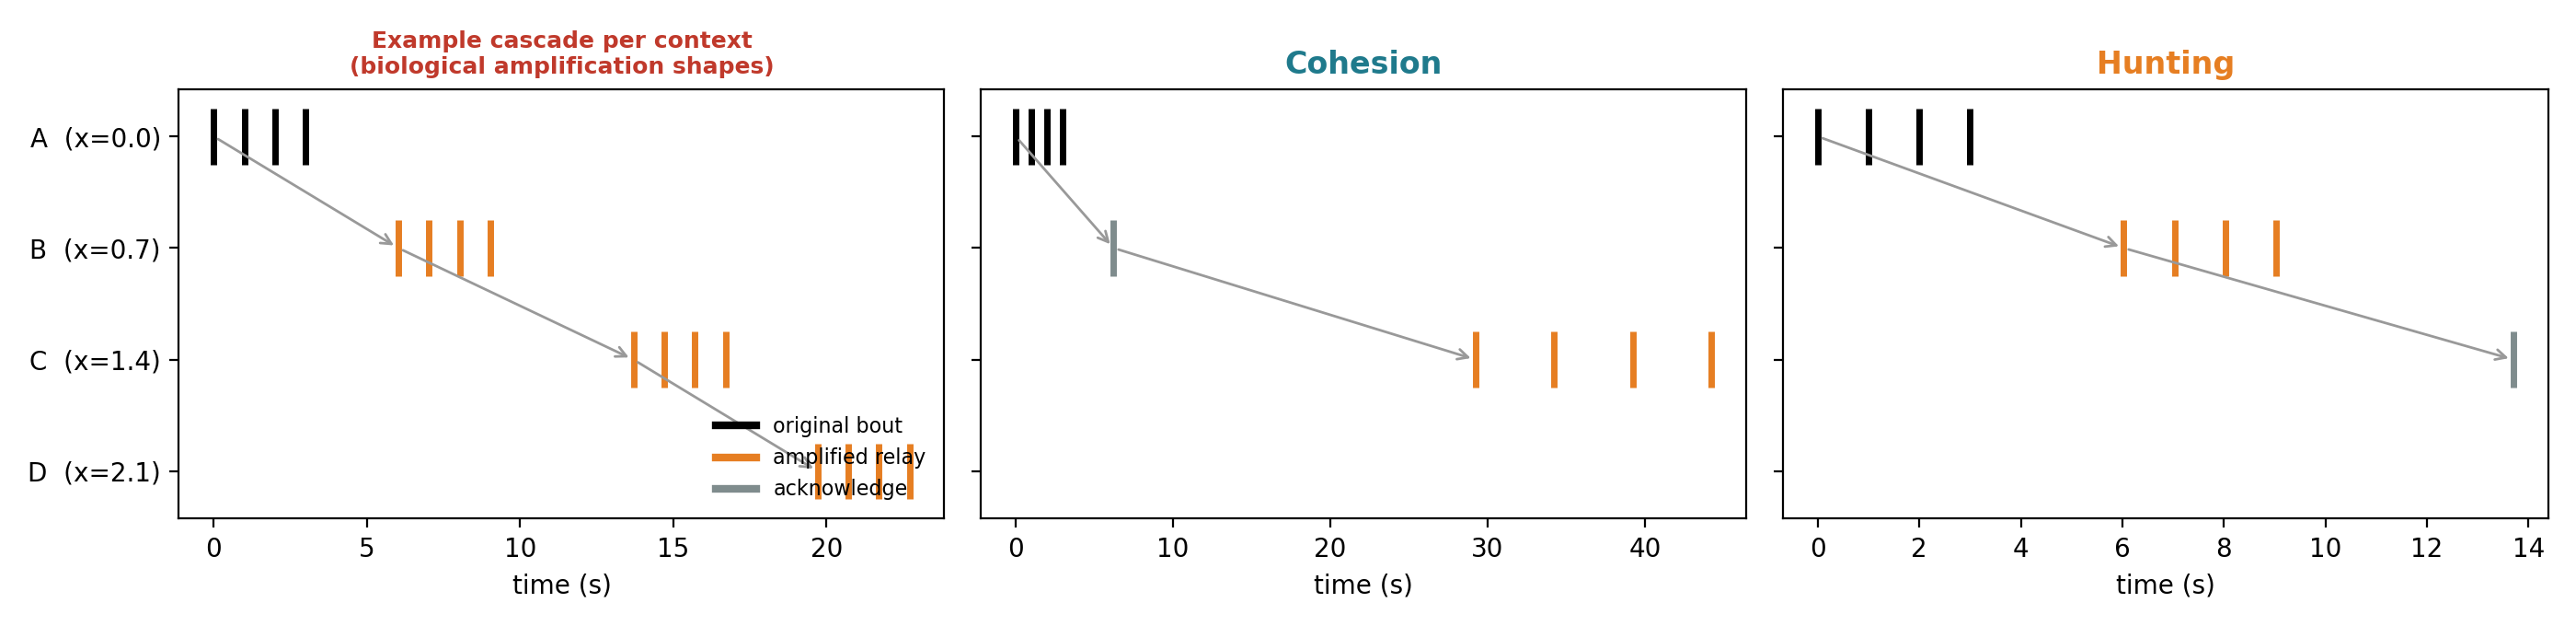
\includegraphics[width=\textwidth]{fig1_example_cascade.png}
\caption{\textbf{Example cascade per context (Model 1, full biological model).}
Each row represents one hyena (A to D). Vertical ticks mark individual whoops; black = original
bout, orange = amplified relay, grey = acknowledgement. Arrows show the relay chain.
The panels illustrate possible relay chains under the amplification shapes that differ between contexts. Hunting is shown for completeness; it is not included in the primary predictions.}
\label{fig:cascade}
\end{figure}

\begin{figure}[h]
\centering
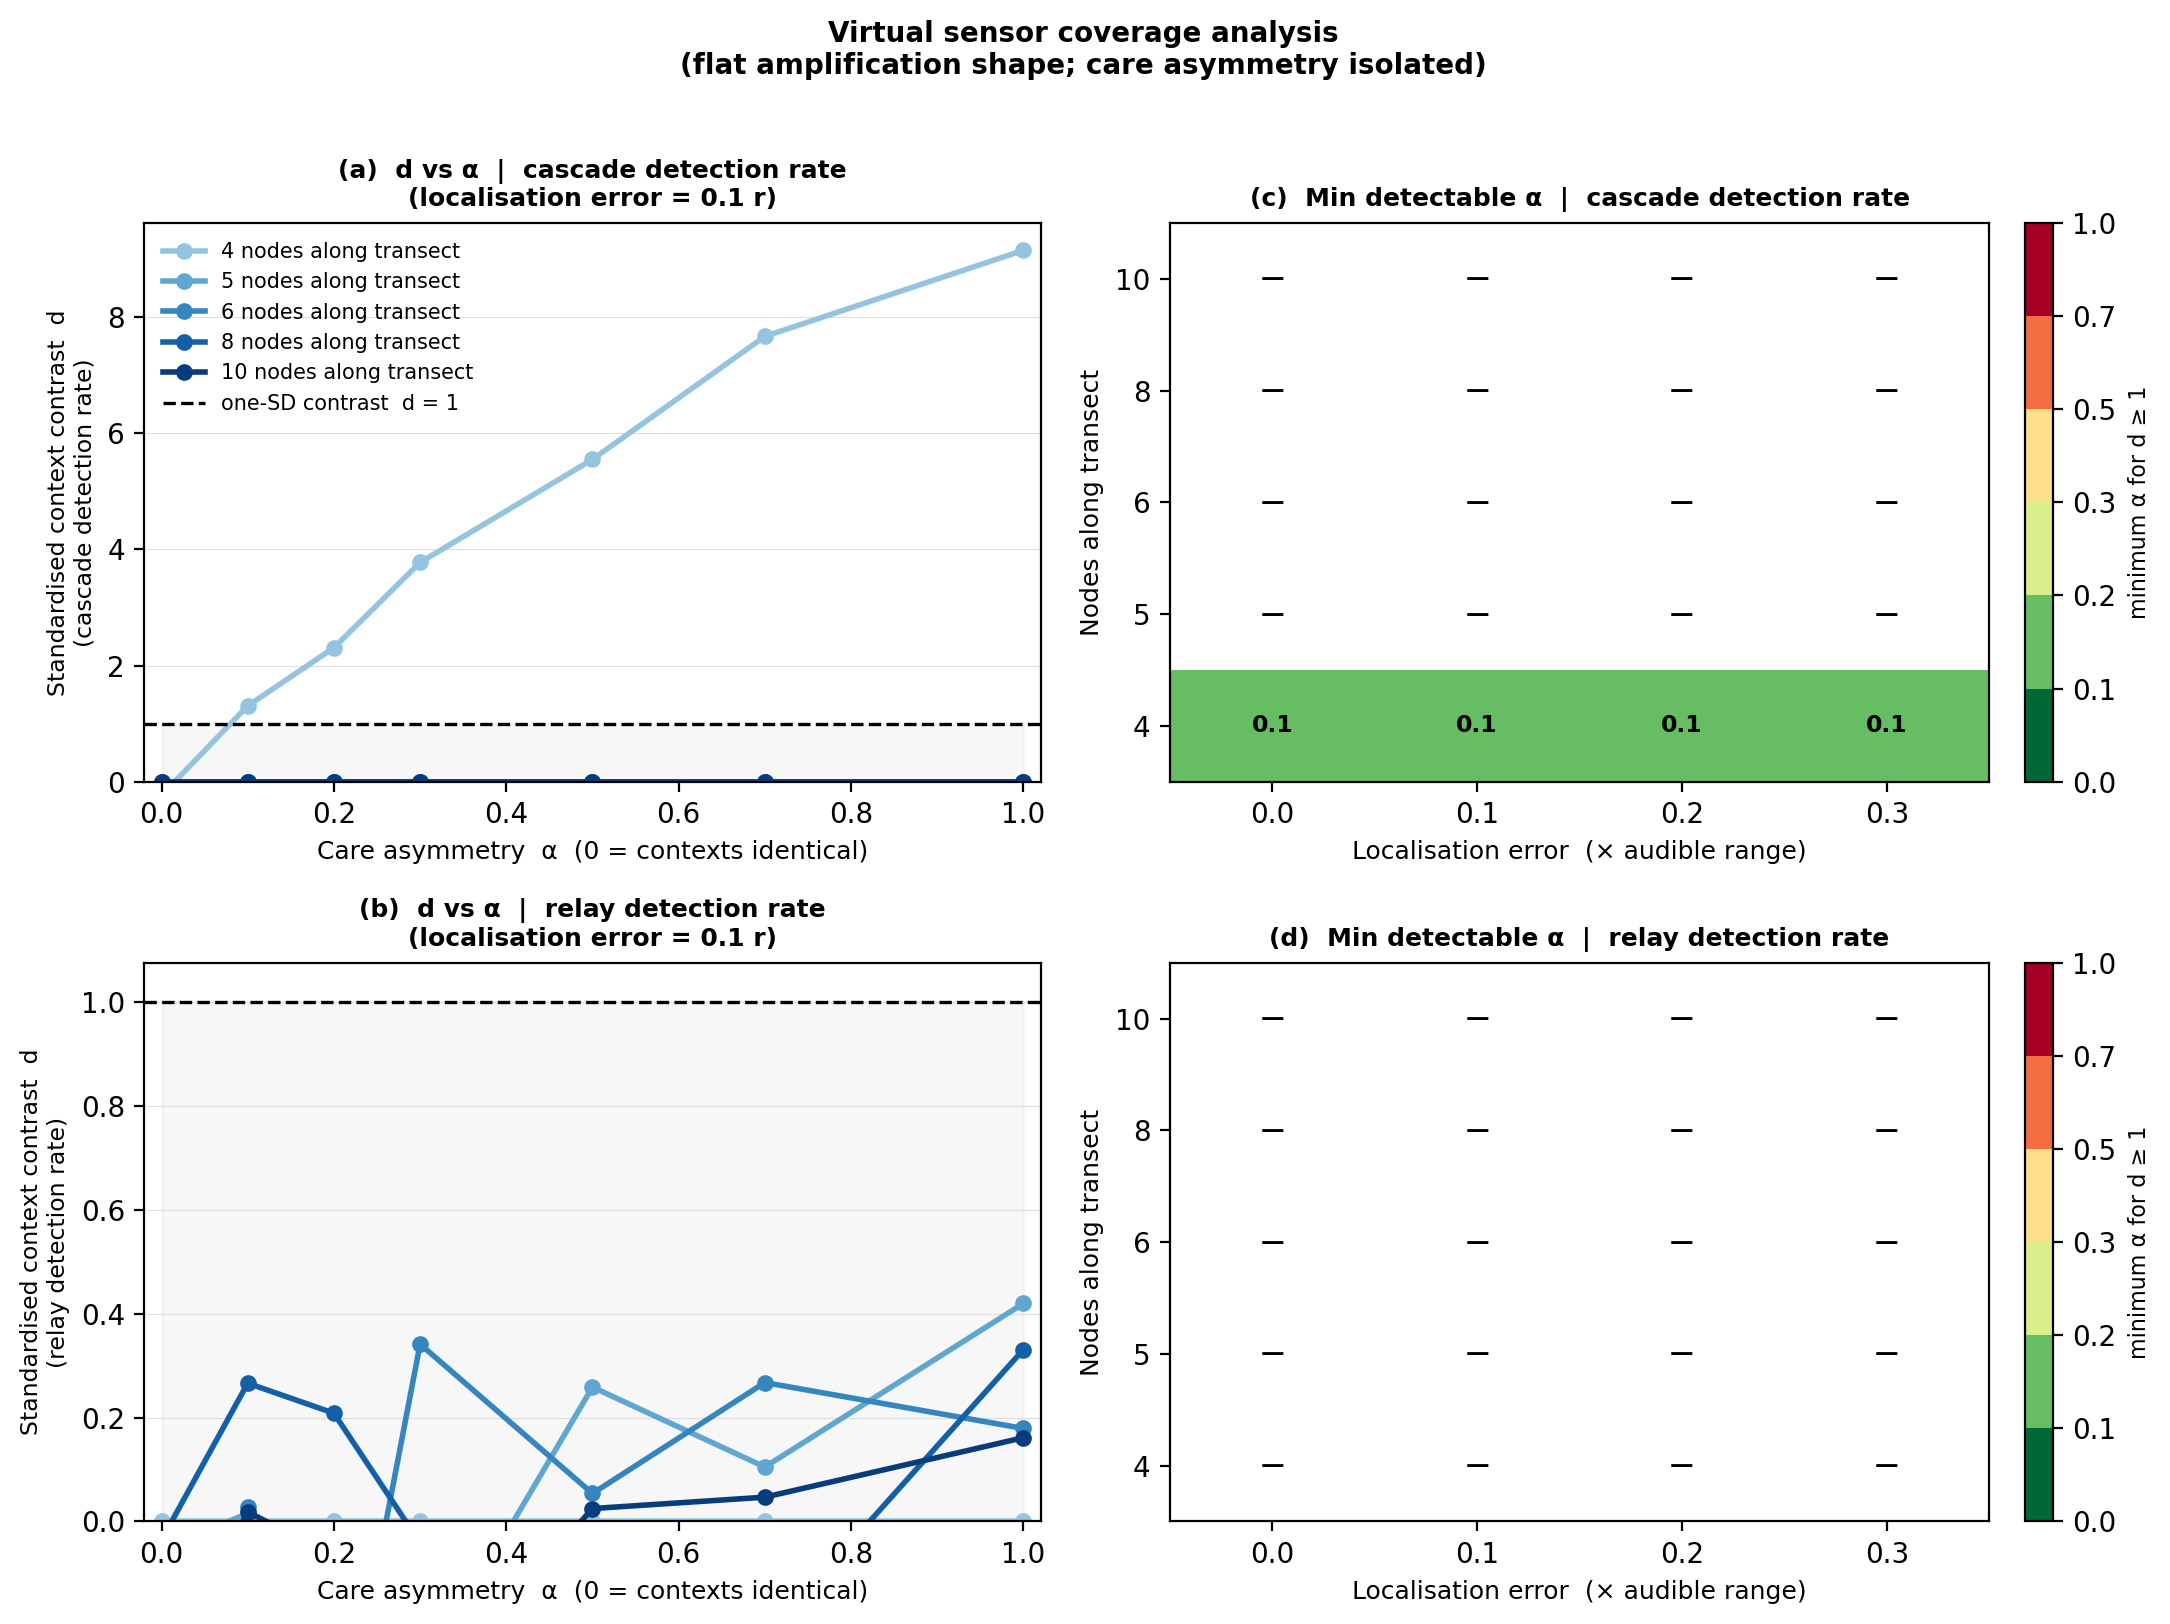
\includegraphics[width=\textwidth]{fig2_sensor_coverage.png}
\caption{\textbf{Virtual sensor coverage analysis (Model 1, flat amplification
shape; care asymmetry isolated).}
Top row: standardised context contrast $d$ for cascade detection rate (a) and
relay recovery rate (b) as a function of care asymmetry $\alpha$, for each number
of nodes along the transect (localisation error fixed at $0.1\,r$). The dashed line
shows the descriptive one standard deviation threshold, $d=1$.
Bottom row: minimum $\alpha$ reaching this threshold as a heatmap over grid density
and localisation error for cascade detection (c) and relay recovery (d). Since
localisation error does not affect whether a call is detected, its effect is
expected only for relay recovery. The threshold is descriptive, not a statistical
significance criterion.}
\label{fig:sensor}
\end{figure}

%%
\section*{Model 2: rank, movement and care}
%%

Four hyenas move in a $3r \times 3r$ arena. Rank 0 represents the highest ranked
individual. They follow a Gaussian random walk (s.d.\ $0.08\,r$ per step), with
reflecting boundaries at the arena walls. At each time step, a randomly chosen
hyena produces an urgent bout with probability 0.3, and a cascade runs.
Every replier moves 0.3 of the way toward the hyena it answered. Care weight
$c_{ij}$ (listener $i$, caller $j$) multiplies $p_{\text{reply}}$:

\begin{center}\small
\begin{tabular}{lll}\toprule
Context  & $c_{ij}$                     & Meaning\\\midrule
Defence  & 1.0 if $i$ top, else 0.8     & Support across the clan\\
Cohesion & 1.0 if $j$ top, else 0.3     & Strong bond with top; little care among subordinates\\
Hunting  & 0.5 for all $i,j$            & Exploratory; not part of P1--P4\\
\bottomrule
\end{tabular}
\end{center}

\textbf{Important framing.} The differences in response probability between ranks in Fig.~\ref{fig:rank} arise
directly from the CARE matrices used in the model. They show what these assumed
rules produce, but they do not establish that the same rules operate in real hyena
clans.

\textbf{On network centrality (P3, P4).} The current version of Model~2 does not calculate network centrality. It includes
only four individuals and is intended to explore how the assumed differences in
response rules between ranks affect participation. It does not represent the
structure of a vocal network across a whole clan. To test P3 and P4, I would need
to run a separate simulation with a larger group and analyse the networks from
individual cascade episodes, rather than pooling all interactions into one network.
The current simulation therefore does not test the centrality predictions.
Fig.~\ref{fig:pam} shows only cascade detection and relay recovery rates.

\textbf{Results (Fig.~\ref{fig:rank}, Fig.~\ref{fig:pam}).}
P(answered) and P(relay) by rank (Fig.~\ref{fig:rank}) show that defence produces
responses across the clan regardless of caller rank (${\sim}68\%$ answered), while cohesion
shows a strong rank asymmetry: ${\sim}58\%$ of the top animal's bouts are answered
but only ${\sim}21\%$ of subordinates'. This difference follows from the different CARE matrices used in the model. The
virtual sensor analysis in Fig.~\ref{fig:pam} shows the proportion of calls detected
and the proportion of true relay episodes recovered at different levels of
localisation error and grid density for each context. Localisation error affects
relay recovery because the estimated positions must preserve the successive
audible range links.

\begin{figure}[h]
\centering
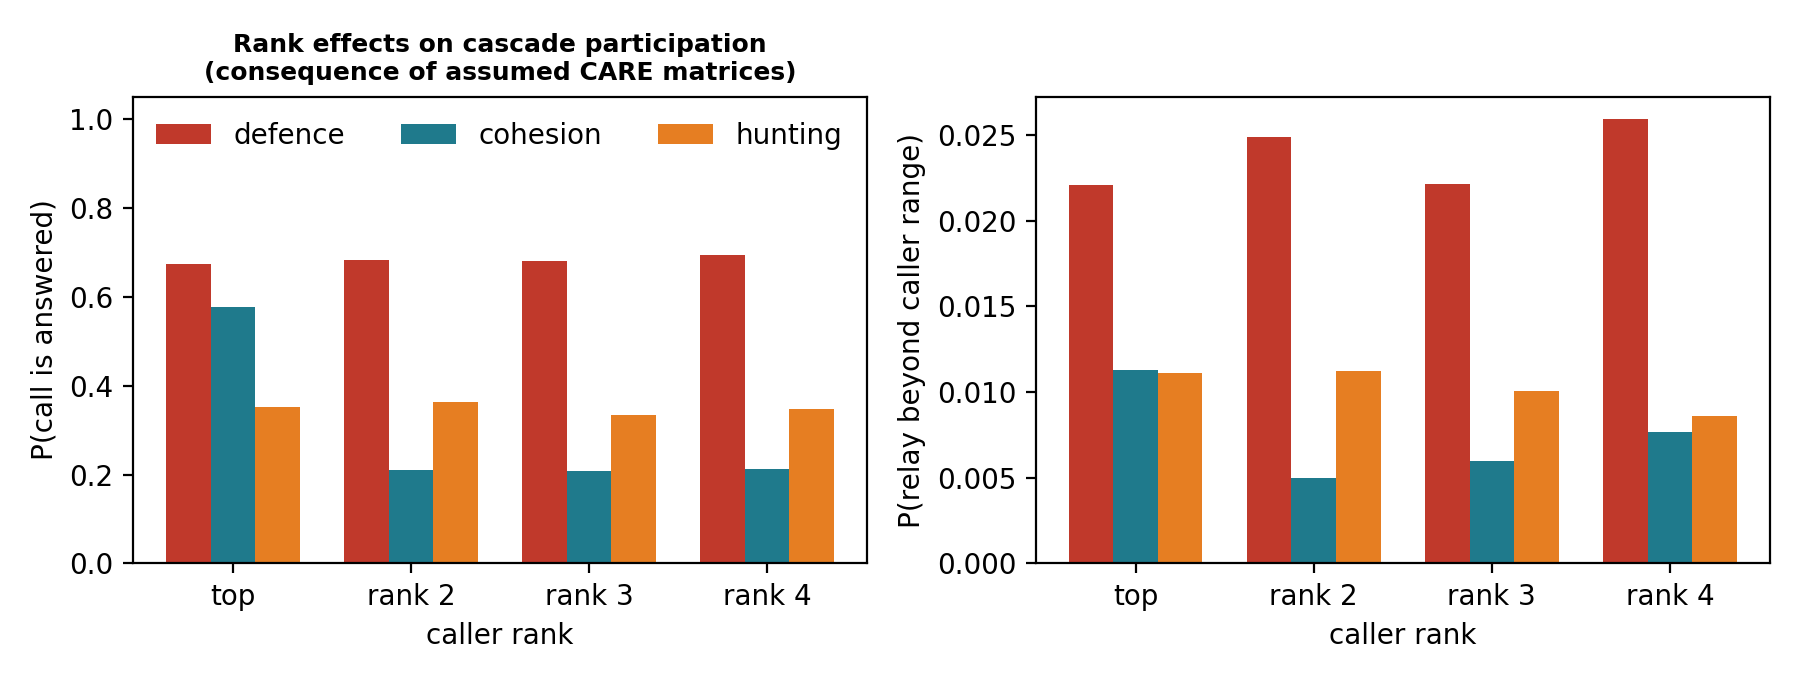
\includegraphics[width=0.8\textwidth]{fig1_rank_responses.png}
\caption{\textbf{P(call answered) and P(relay) by caller rank (Model 2).}
Bars show means across 100 replicates. Defence shows little rank effect; cohesion
shows a strong asymmetry favouring the caller with the highest rank. These patterns follow from the assumed CARE matrices and are not independent
findings about real hyenas.}
\label{fig:rank}
\end{figure}

\begin{figure}[h]
\centering
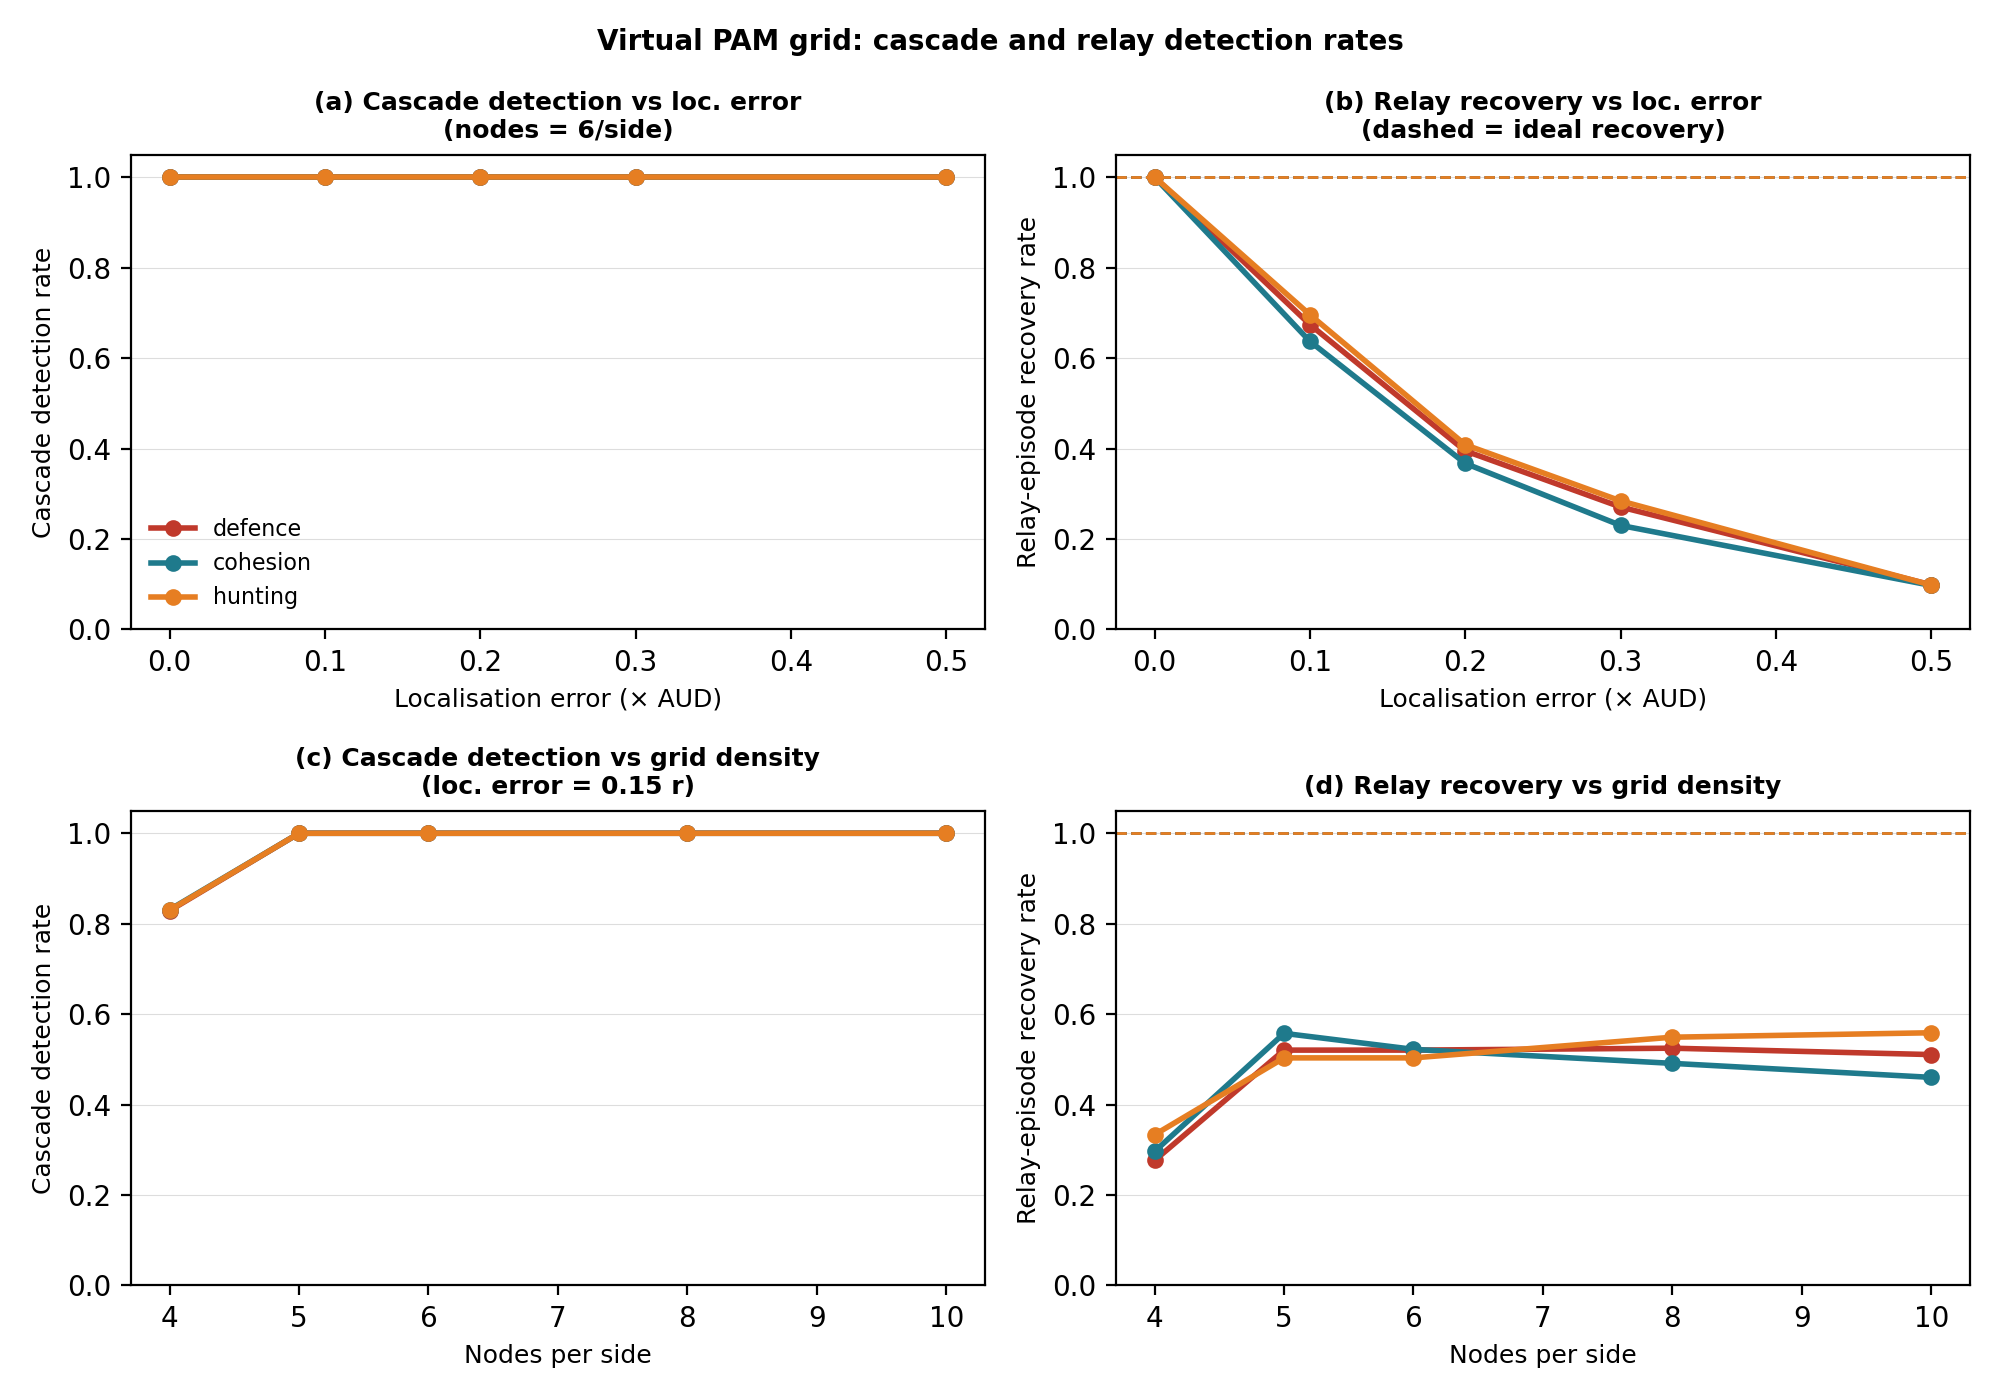
\includegraphics[width=\textwidth]{fig2_pam_detection.png}
\caption{\textbf{Virtual sensor grid detection rates (Model 2).}
Cascade detection rate (proportion of all calls detected) and recovery of relay episodes
rate (proportion of episodes containing a true relay for which the complete relay
path is recovered) as functions of localisation error (top row, nodes fixed at 6 per side)
and grid density (bottom row, localisation error fixed at $0.15\,r$). Detection
depends on true spatial coverage; localisation error affects whether the estimated
positions preserve the relay path. Dashed lines indicate ideal relay recovery.}
\label{fig:pam}
\end{figure}

%%
\section*{Limitations}
%%

\textbf{Structural.}
Both models encode hypotheses as rules rather than testing them. All parameters are
set for illustrative contrast and are not fitted to empirical data.

\textbf{Group and spatial structure.}
Four individuals in a small arena do not represent a Mara clan territory
(13--76\,km$^2$) or clan size (up to 125 individuals). Network centrality
predictions (P3 and P4) are not evaluated in this version of the model.

\textbf{Sensor model.}
The virtual sensor checks spatial coverage and adds Gaussian error to the estimated
positions. It does not simulate TDOA localisation. In Model~1, nodes are arranged
along a transect. In Model~2, nodes form a two dimensional grid, and grid density
is reported as the number of nodes per side. Localisation error affects relay path
recovery, but not call detection.

\textbf{Context assignment.}
In the field analysis, social context will be assigned from direct behavioural
observation, not from interval between whoops alone. The interval between whoops is extracted
separately as the urgency measure.

\end{document}
